\subsection{Beleuchtung}
\label{subsec:Beleuchtung_2}

Damit die Maschine erkennbar ist und auch Eindruck schindet, wurde ein auffallendes Mittel benötigt. Dazu eignet sich ein LED-Band, am besten, wenn es noch verschiedenfarbig ist. Dazu ist einerseits das LED-Band von Nöten und die geeignete Ansterung dazu. Für die Cocktailmaschine wurde festgelegt, dass der LED-Streifen die benötigten Wirderstände für die LED's schon integriert hat und die Ansteuerung folglich direkt über MOSFET's geschehen kann. Der Aufbau ähnelt dann dem in Abbildung \ref{fig:LED1} gezeigten Schaltung. Der Streifen ist Rot eingerahmt, die LED's und Widerstände befinden sich auf dem Band und die zu sehenden Fähnchen für R, G, B und W führen zum Mikrocontroller. Es können auch mehrere Bänder parallel geschaltet werden, wie in Abbildung \ref{fig:LED1} ersichtlich ist.

\begin{figure}[h!]
\center
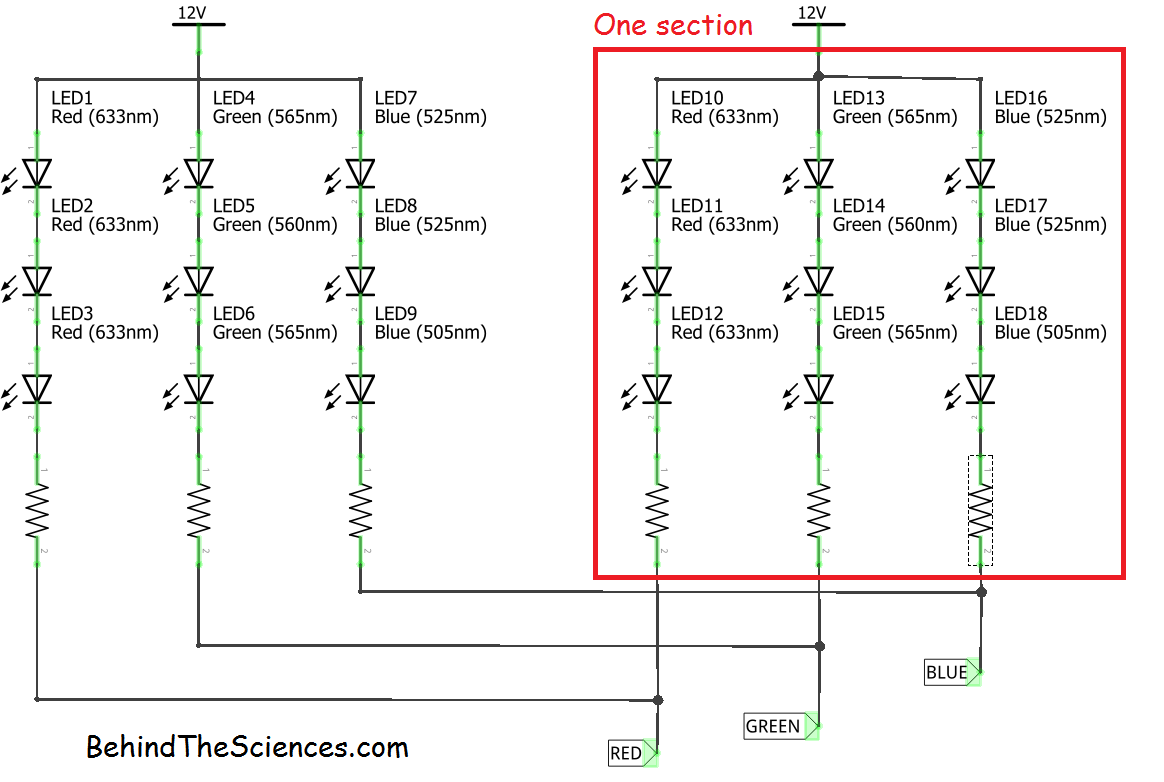
\includegraphics[width = 0.5\textwidth]{graphics/Schema_LED1}
\caption{LED Beispiel. \cite{behindthesciences_rgb_2017}}
\label{fig:LED1}
\end{figure}

\paragraph{Schema}\mbox{}

Abbildung \ref{fig:Schema_LED} zeigt den Schaltungsaufbau der LED-Steuerung. Damit die LED's angesteuert werden können, braucht es ein Bauteil welches mit einer 5V-Ansteuerung 12V schalten können. Dazu wird der Selbe MOSFET verwendet wie schon bei den Pumpen in Kapitel \ref{subsubsec:Pumpen}. Über die Widerstände an den Gates wird der Strom zum Schutz des Gates begrenzt. Ausserdem verhindern sie ein allfälliges Oszillieren. Die Leitungen führen direkt auf den Klemmblock für die LED-Streifen. Parallel dazu wurde noch für jede Lichtfarbe ein Kontroll-LED installiert, welches es ermöglicht auch ohne LED-Band etwas zu programmieren und ersichtlich zu machen.

\begin{figure}[!h]
\center
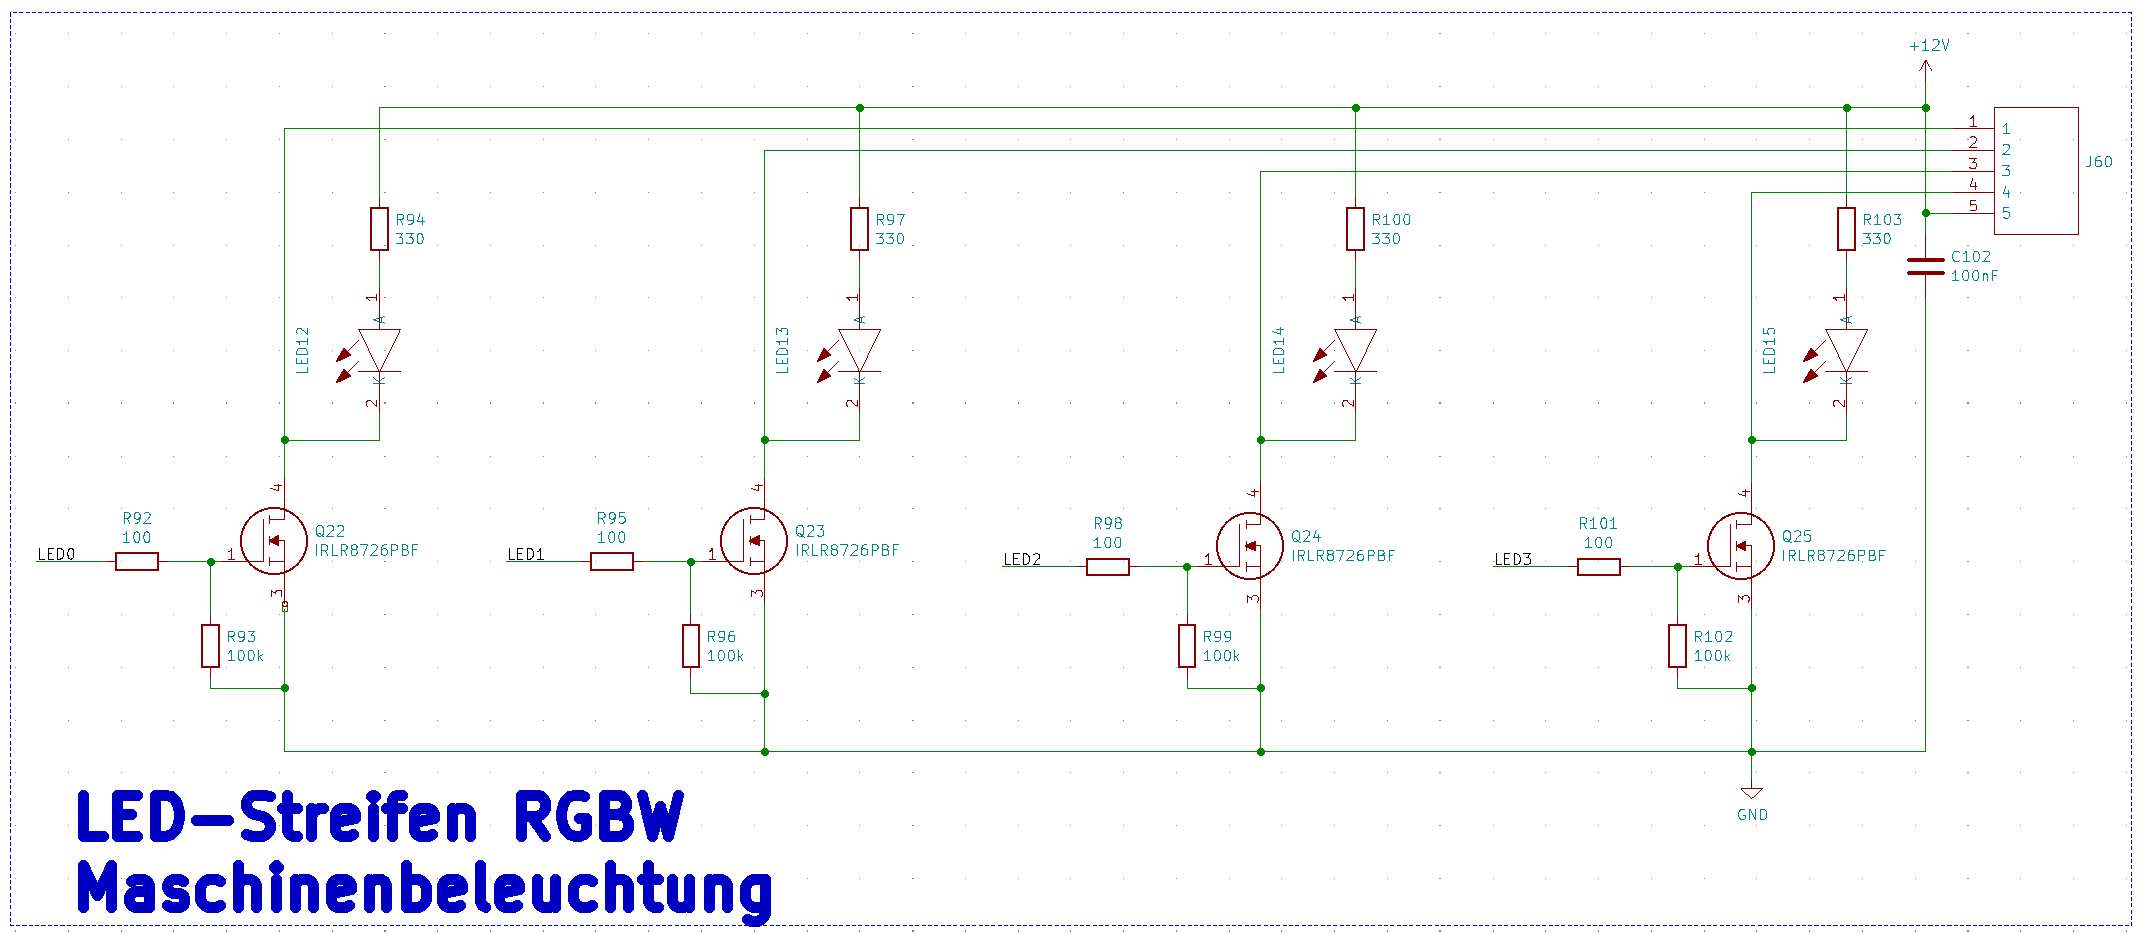
\includegraphics[width =  \textwidth]{graphics/Schema_LED}
\caption{Schema der LED-Ansteuerung}
\label{fig:Schema_LED}
\end{figure}
\newpage
\paragraph{Funktionsbeschrieb der Schaltung}\mbox{}

Bei Licht handelt es sich bekanntlich um elektromagnetische Wellen, welche im sichtbaren Wellenlängen-Bereich liegen. Dabei gibt es vier Hauptfarben: Rot, Grün, Blau und Weiss. Zwar kann Weiss auch aus einer Kombination aller drei Farben erstellt werden, es kommt aber besser mit einer separaten Diode. Das resultierende Licht des Bandes ist eine Überlagerung der Wellenlängen. Diese Überlagerung kann vom Mikrocontroller über den Duty-Cycle eines PWM-Signals gesteuert werden. So lassen sich mit dem Licht aus den Grundfarben praktisch alle Farben mischen.